\subsubsection{Protocolo \textbf{ICMP}}

\textbf{ICMP}\cite{rfc792} (\emph{Internet Control Message Protocol}) es un protocolo que
forma parte de la arquitectura \textbf{TCP/IP} pensado para mensajes de control
de Internet. Se utiliza en situaciones, y distintos própositos como

\begin{itemize}
	\item Cuando un datagrama no puede alcanzar su destino
	\item Cuando un router no tiene la capacidad de forwardear este paquete
	\item Redirigir el host hacia una ruta más corta para el envio del paquete
	\item Se quiere comprobar que una maquína esta viva (\textbf{ping})
	\item Se quiere saber la ruta a un determinado host (\textbf{traceroute})
\end{itemize}

\subsection{Algoritmo Traceroute}

\subsubsection{Descripción del algoritmo}

\begin{figure}[ht]
	\begin{center}
		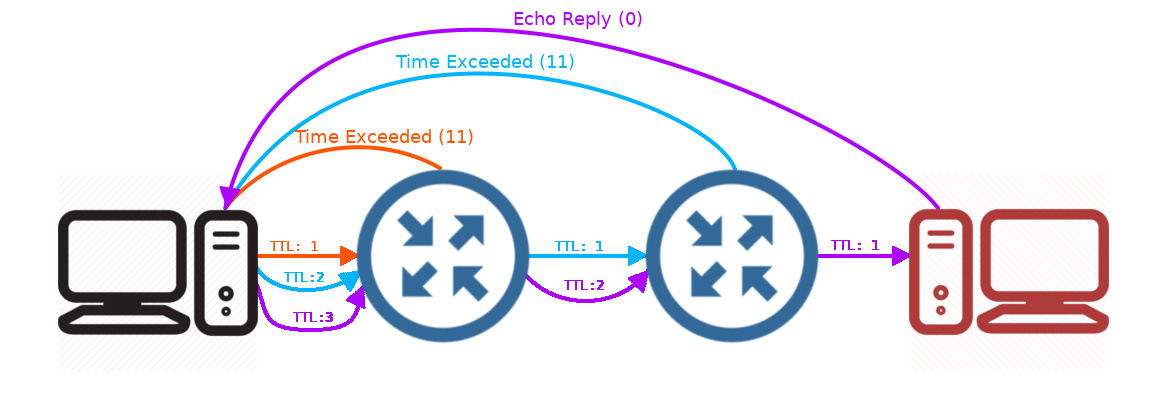
\includegraphics[width=0.8\columnwidth]{imagenes/diagrama_1.jpg}
		\caption{Diagrama de envio de paquetes del algoritmo}
		\label{fig:diagramasimple}
	\end{center}
\end{figure}

Sea $S$ el host que desea enviar el paquete y $T$ el host destino.
El algoritmo consiste en enviar desde $S$ al host de destino $T$ paquetes
\emph{echo} con el campo $TTL=i$ en el datagrama \textbf{IP} para $i=1 \dots
MAX\_HOPS$ o hasta que se haya alcanzado al host $T$. Cada vez que el paquete
es forwardeado por un gateway al próximo host (Next Hope), este decrementará el
valor de este TTL. Cuando el valor llegue a cero el último gateway, llamemoslo
$M$, le informará mediante un paquete \textbf{ICMP} que el host de destino $T$
es inalcanzable (ver figura \ref{fig:diagramasimple}), obteniendo a su vez $S$ con esto, la \textbf{IP} de $M$ como
tambien la estimación del \textit{Round
Trip Time} (RTT) a este host $M$, y como se explicará luego el $RTT$ del enlace
del anterior gateway hasta este. Como esto se realiza reiteradas veces, en
cada paso, aumentando el TTL se llegan a conocer, en teoría, todos los
gateways, desde $S$, intermedios hasta llegar al destino $T$.

\subsubsection{Posibles problemas en la vida real}


Esto brinda en teoria una ruta efectiva bajo los supuestos de que
las rutas intermedias de forwarding se mantienen invariantes en el tiempo. En
la practica, esto no es usual dando a lugar a los siguientes inconvenientes

\begin{itemize}
	\item En cada salto es posible que cambien los gateways anteriores y siendo
	ademas imposible de detectar. (esto se puede ver en la figura \ref{fig:diagramareal})
	\item El \textbf{RTT} estimado incluye al tiempo de encolamiento (es por esto
	que se le llama estimado) provocando una desviación significativa en las
	mediciones.
\end{itemize}

\begin{figure}[ht]
	\begin{center}
		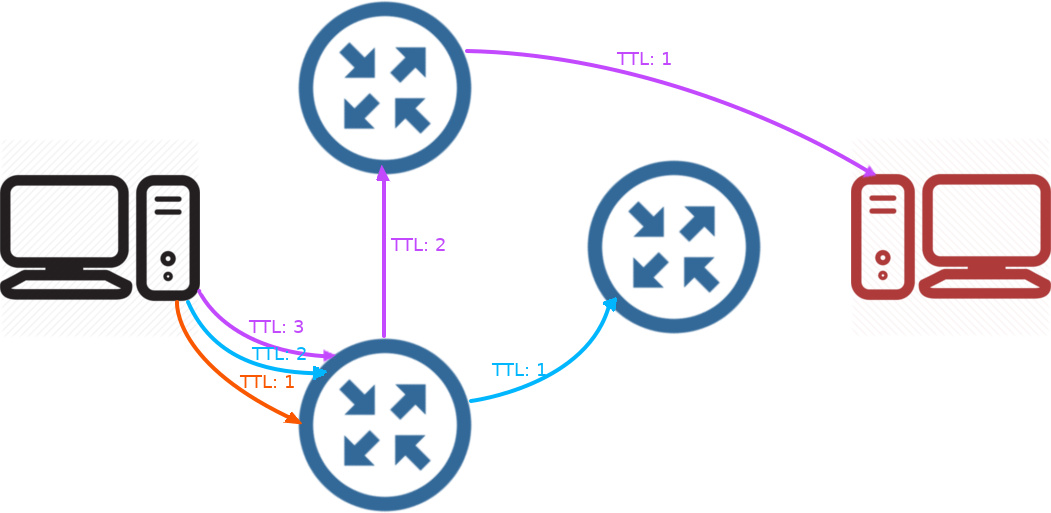
\includegraphics[width=0.8\columnwidth]{imagenes/diagrama_2.jpg}
		\caption{Diagrama de envio de paquetes del algoritmo}
		\label{fig:diagramareal}
	\end{center}
\end{figure}

Para solventar este tipo de problemas, para cada $TTL$ se envian varios paquetes
para luego obtener un valor promedio de $RTT$ mas significativo que el de un
solo intento, como a su vez, devolver solo la \textbf{IP} que respondió con mas
frecuencia.

Para calcular el $RTT$ del enlace promedio, se realiza la resta
del promedio del $RTT$ total obtenido en esta etapa con el promedio del $RTT$ total
de la etapa anterior.
Es decir

\begin{equation}
	\Delta RTT_{i} = \left\{
		\begin{array}{cl}
			\overline{RTT_{0}} & \mbox{si } i = 0\\
			\overline{RTT_{i}} - \overline{RTT_{i-1}} & \mbox{si } i > 0
		\end{array}
		\right.
\end{equation}

Cuando los tiempos de encolamiento y las rutas son invariantes en el tiempo
esta magnitud física siempre es positiva. Pero como, se mencionó anteriormente, esto
no siempre es así. La medida que toma el algoritmo en los casos cuando
$\Delta RTT_{i} < 0$ es la de descartar el
gateway y considerarlo como que forma parte del enlace.

\subsection{Determinación de enlace intercontinental}

El objetivo de este algoritmo además de brindar la ruta, es el de detectar de
forma automática, cuando un enlace intermedio por el que es forwardeado el
paquete es uno que cruza dos continentes, debiendose esto posiblemente a
que el cable fisicamente es transatlantico (cables submarinos que cruzan el
atlantico). Una vez calculado el $\Delta RTT_{i}$ de cada enlace hasta llegar
al ultimo host se realiza la normalización (se los lleva a la distribución normal)
el valor de cada uno con la siguiente formula.

\begin{equation}\label{eq:z}
	Z_{i} = \lvert\frac{\Delta RTT_{i} - \overline{\Delta RTT}}{\sigma \left(\Delta RTT \right)}\rvert
\end{equation}

Este valor $Z_{i}$ es de vital importancia ya que nos dice, estadisticamente,
para $\Delta RTT_{i}$ cuantas desvaciones estandar se aleja de la media.
Combinando esto con el trabajo de John M. Cimbala\cite{cimbala} nos da una forma de
detectar cuando en un muestreo se presentó un outlier dependiendo también de la
cantidad de muestras. La aplicación que tiene en el trabajo realizado es que se
termina identificando cuando el $RTT$ del enlace es atípicamente alto los que nos
proporciona un sofisticado criterio para detectar los enlaces
intercontinentales como se comprobará mas adelante en las siguientes secciones.
